\chapter{Einleitung} 
Die Idee objektorientierter Programmierung kam erstmals Ende der 1950er Jahre auf, als Systeme aus der realen Welt in Form von Programmen abgebildet werden sollten. Viele Systeme aus der realen Welt bestehen aus hunderten oder sogar tausenden miteinander interagierenden Teilen. Um dieses Verhalten abbilden zu können, mussten auch die Programmsysteme in kleine, handhabbare Teile zerlegt werden: in Objekte \cite{history}.

Objekte sind Programmeinheiten, die einen eigenen Zustand besitzen und mit anderen Objekten interagieren können. So wie reale Objekte von uns klassifiziert werden (zum Beispiel als ``Tisch'' oder ``Stuhl''), gibt es auch in der objektorientierten Programmierung Klassen, die Objekte mit ähnlichen Eigenschaften zusammenfassen. Sie sind wie ein Bauplan, der das grundlegende Verhalten der Objekte anhand von Attributen (Feldern) und Methoden festlegt.

Objektorientierte Programmierung erlaubt uns eine Verringerung der Komplexität eines Problems: Anstatt das komplette Verhalten eines Systems auf einmal darzustellen zu müssen, wird es aufgeteilt in kleine, übersichtliche Teilsysteme und deren Interaktion untereinander.

Ein wichtiges Kernkonzept von objektorientierter Programmierung ist Vererbung: die Fähigkeit einer Klasse, Verhalten einer anderen Klasse zu übernehmen, ohne den Code explizit noch einmal schreiben zu müssen. Gibt es beispielsweise in der Klasse \texttt{A} ein Feld oder eine Methode \texttt{a}, so hat auch jedes Objekt einer Klasse \texttt{B}, die von \texttt{A} erbt, diese Eigenschaft (Abb. \ref{inheritance}).

\begin{figure}[h]
\centering
 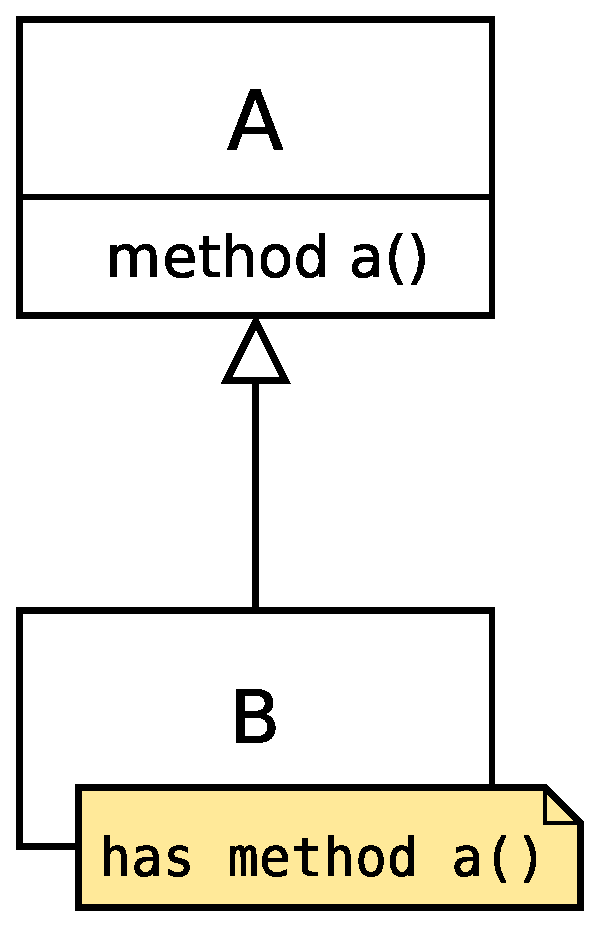
\includegraphics[scale = 0.3]{pictures/inheritance}
 \caption{Vererbung einer Methode.}
 \label{inheritance}
\end{figure}

Erbt eine Klasse von mehreren anderen Klassen, so nennt man das Mehrfachvererbung. Mehrfachvererbung war lange ein umstrittenes Thema in der objektorientierten Welt \cite{mi1}\cite{mi2}, denn sie kommt mit einer Herausforderung: Wie geht man damit um, wenn zwei gleichbenannte Methoden (oder Felder) geerbt werden? Eine sehr bekannte Ausprägung dieses Problems nennt sich das Diamond-Problem \cite{dp}. Es erhält seinen Namen von der Tatsache, dass die Vererbungshierarchie die Form einer Raute (englisch \emph{rhombus} oder \emph{diamond}) hat (Abb. \ref{diamond}):
Eine Klasse \texttt{D} erbt von zwei anderen Klassen \texttt{B} und \texttt{C}, die eine gemeinsame Superklasse \texttt{A} haben. Diese Superklasse hat ein Element (hier die Methode \texttt{a()}), das an beide Subklassen \texttt{B} und \texttt{C} vererbt wird und damit schlussendlich zweimal an \texttt{D}. Das Diamond-Problem ist nun die Fragestellung, wie die Klasse \texttt{D} damit umgeht.

\begin{figure}[h]
\centering
 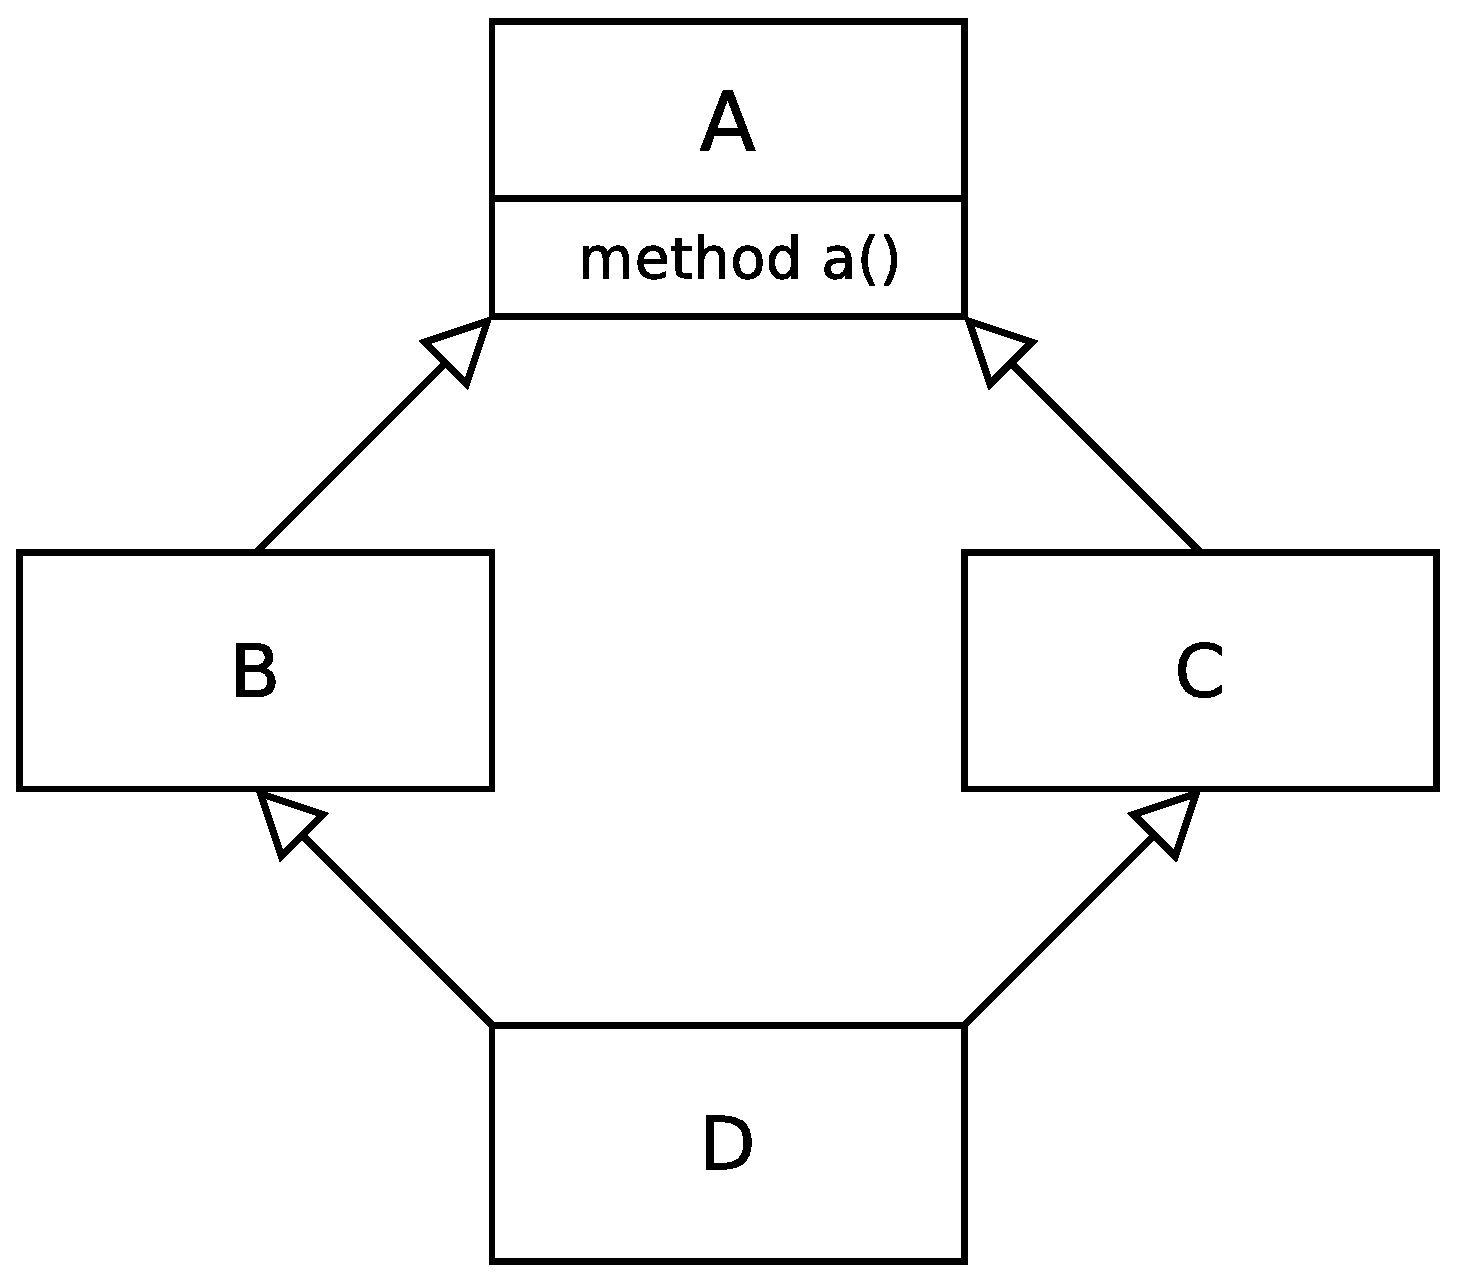
\includegraphics[scale = 0.3]{pictures/diamond}
 \caption{Das Diamond-Problem.}
 \label{diamond}
\end{figure}

Dafür haben sich im Laufe der Zeit in verschiedene Programmiersprachen (im folgenden: Sprachen) verschiedene Herangehensweisen entwickelt \cite{wikipedia}, die sich grob in sieben Strategien unterteilen lassen:

\begin{enumerate}
 \item Mehrfachvererbung wird nicht unterstützt. Als Alternative werden teils Mixins oder Traits genutzt. Beispiel: Java bis Version 7.
 \item Es ist nicht erlaubt, mehrdeutige Eigenschaften zu verwenden. Wenn in der Klasse \texttt{D} die Methode \texttt{a()} aufgerufen wird, so führt das zu einem Fehler. Beispiel: Go, Java 8.
 \item Zu vererbende Eigenschaften werden per Hand gewählt. Die Klasse \texttt{D} kann sich also entscheiden, entweder \texttt{B.a()} zu erben oder \texttt{C.a()}. Beispiel: Eiffel.
 \item Gleichbenannte Eigenschaften werden umbenannt. \texttt{D} würde zwei Methoden \texttt{ba()} und \texttt{ca()} erben. Beispiel: Eiffel, Logtalk.
 \item Man kann qualifiziert auf die Eigenschaften zugreifen. In \texttt{D} kann man dann mit \texttt{B.a()} oder \texttt{C.a()} die Methode aufrufen. Beispiel: C++, OCaml.
 \item Eigenschaften werden nach Präzedenz geerbt. Die Superklassen werden in eine bestimmte Reihenfolge (Präzedenzliste) gebracht und bei gleichbenannten Eigenschaften wird immer nur dasjenige geerbt, das in der Präzedenzliste zuerst kommt. Wenn wir beispielweise die Klassen in die Reihenfolge \texttt{D,B,C,A} bringen, so würde die Eigenschaft je nach Implementierung entweder von \texttt{B} oder direkt von \texttt{A} geerbt, jedoch nur einmal. Beispiel: Common Lisp, Perl, Python.
 \item Kombination aller gleichbenannten Eigenschaften. Der Programmierer kann angeben, wie die geerbten Eigenschaften kombiniert werden sollen. Das funktioniert gegebenfalls sogar für indirekte Superklassen. Haben \texttt{A} und \texttt{B} eine gemeinsame Eigenschaft, dann gehen beide in die Kombination mit ein. Beispiel: Common Lisp, Eiffel.
\end{enumerate}

% Für einen möglichst einfachen Einstieg in die Lehre von Mehrfachvererbung bietet sich Kategorie 6 am meisten an: Die Konfliktlösung passiert automatisch. Es reicht, eine Vererbungshierarchie anzugeben und den Rest übernimmt die Sprache. 

Racket nutzt die erste Strategie. Mehrfachvererbung wird nicht unterstützt.

Das Common Lisp Object System (CLOS) \cite{keene} vereint die Ansätze 6 und 7: Wird nichts anderes angegeben, so wird die Eigenschaft der Klasse mit der höchsten Präzedenz vererbt; der Programmierer hat jedoch für Methoden alternativ auch die Möglichkeit, eine Kombinationsart anzugeben. Diese Art der Mehrfachvererbung bietet auch einen einfachen Einstieg für die Lehre. Die Konfliktlösung ist automatisiert. Es reicht, eine Vererbungshierarchie anzugeben und den Rest übernimmt die Sprache. Gleichzeitig erhält der Programmierer durch Angabe einer Kombinationsart auch selbst die Möglichkeit der Kontrolle.

Die Funktionsweise von CLOS ist sehr ausführlich in dem Buch ``Object-oriented programming in Common Lisp. A programmer's guide to CLOS'' von Sonya E. Keene \cite{keene} dokumentiert. Einen Blick hinter die Implementierung werfen Gregor Kiczales, Jim Des Rivieres und Daniel Gureasko Bobrow mit dem Werk ``The art of the metaobject protocol'' (AMOP) \cite{amop}. Sie zeigen wie eine objektorientierte Sprache auf Basis von Lisp, Makros und Metaobjekten implementiert werden kann. 

Das Hinzufügen von Mehrfachvererbung zu einer bestehenden objektorientierten Sprache ist jedoch bisher wenig dokumentiert. 

\section{Motivation} 
An der Universität Hamburg gliedert sich die Lehre zur Softwareentwicklung in zwei Abschnitte. Im ersten Abschnitt werden in den Veranstaltungen ``Softwareentwicklung I'' und ``Softwareentwicklung II'' die Grundlagen für das Programmierverständnis gelegt. Die Studierenden erhalten einen  Einblick in imperative und objektorientierte Programmierung in Java nach dem Objects-First-Ansatz \cite{objectsfirst}.

Anschließend bieten die optionalen Module ``Softwareentwicklung III: Funktionale Programmierung'' sowie ``Softwareentwicklung III: Logikprogrammierung'' zusätzlich die Möglichkeit, zwei weitere  Programmierparadigmen kennenzulernen: funktionale Programmierung am Beispiel von Racket und logikbasierte Programmierung am Beispiel von Prolog.

Racket ist ein Dialekt der funktionalen Sprache Lisp. Genau wie Lisp hat Racket einen funktionalen Kern und ist gleichzeitig eine Mul\-ti\-pur\-pose-Spra\-che. Racket erlaubt es, neben dem funktionalen Stil auch imperative, obkjektorientierte und sogar logikbasierte Programme zu schreiben. Im Rahmen der Lehrveranstaltung werden daher auch diese Möglichkeiten aufgezeigt. 

Racket bietet zwei Arten, objektorientiert zu programmieren: ein integriertes Objektsystem, das sehr ähnlich zu Java ist, und eine Implementierung des Common Lisp Object Systems (CLOS), das eine eher funktionale Sicht auf die Objektorientierung hat. 

Da die Studierenden bereits aus ``Softwareentwicklung I'' und ``Softwareentwicklung II'' mit Java vertraut sind, bietet das Objektsystem von Racket kaum neue Lehrinhalte. Aus diesem Grund wird bisher CLOS, das in dem Racketdialekt Swindle implementiert ist, als Lehrinhalt behandelt. 

\section{Problemstellung} 
Für die Implementation von CLOS wird ein so genanntes Metaobjektprotokoll verwendet, in dem Informationen über Klassen und Objekte durch interne Objekte verwaltet werden. In dieser Arbeit soll untersucht werden, ob das Metaobjektprotokoll auch genutzt werden kann, um Verhalten von CLOS zu dem bestehenden Objektsystem von Racket hinzuzufügen. Falls dies möglich ist, soll eine Spracherweiterung von Racket entwickelt werden. 

Die Spracherweiterung kann zukünftig im Rahmen der Lehre des Moduls ``Softwareentwicklung III'' genutzt werden, um Mehrfachvererbung direkt anhand des Objektsystems von Racket zu behandeln. Der Fokus liegt auf lehrrelaventen Konzepten: 
\begin{itemize}
 \item Mehrfachvererbung
 \item Klassenpräzedenz
 \item Methodenkombination
 \item Ergänzungsmethoden
\end{itemize}

% Es ist bisher nicht möglich, diese Paradigmen in vollem Umfang im Objektsystem von Racket zu verwenden. Beide Systeme verwenden außerdem unterschiedliche Objekte, die nicht ohne weiteres miteinander kommunizieren oder ineinander umgewandelt werden können.
% 
% Im Rahmen dieser Arbeit soll eine Racket-Erweiterung entstehen, die Mehrfachvererbung auch im Objektsystem von Racket möglich ermöglicht. Als Anleitung soll die bereits existierende Umsetzung in CLOS dienen. 


\section{Vorgehen}
Um über Mehrfachvererbung in Racket und CLOS reden zu können, werden im Kapitel \textbf{Objektsysteme in Racket} die Sprache Racket und die existierenden Objektsysteme beschrieben. Das Kapitel soll ein Gefühl dafür geben, wie die beiden Systeme zu benutzen sind und Gemeinsamkeiten, Unterschiede und Grenzen aufzeigen.

Anschließend wird im Kapitel \textbf{Entwurf} ein Vorschlag gemacht, auf welche Weise Racket um Mehrfachvererbung erweitert werden kann. 

Im Kapitel \textbf{Analyse der Implementierungsdetails von CLOS} wird anhand der Implementierung von CLOS ergründet, wie das Metaobjektprotokoll genutzt werden kann, um ein bestehendes Objektsystem um die Möglichkeit von Mehrfachvererbung zu erweitern. Es werden relevante Implementierungsdetails von CLOS beschrieben und ihre Anwendbarkeit auf das Objektsystem von Racket evaluiert.

Das Kapitel \textbf{Umsetzung} beschreibt den in dieser Arbeit entstandenen Prototypen und beleuchtet Abweichungen zu CLOS sowie Probleme, die bei der Umsetzung auftraten und wie sie gelöst wurden.

In der \textbf{Auswertung} wird der entstandene Prototyp getestet. Es werden Einschränkungen, die gemacht werden mussten, beleuchtet und ein Fazit über die Eignung des Metaobjektprotokolls zur Erweiterung eines Objektsystems gezogen.

Zum Abschluss werden in \textbf{Zusammenfassung und Ausblick} noch einmal die Ergebnisse zusammengefasst und Möglichkeiten der Erweiterung diskutiert.

\section{Beiliegende CD}
Auf der beiliegenden CD befindet sich eine digitale Version dieser Arbeit sowie der entstandene Prototyp und eine Zusammenstellung der behandelten Beispiele als Racketdateien.

